\section{Experiments}
\label{sec:exp}

We trained the modules first to obtain $Q_i$ before running the inverse
reinforcement learning algorithm. For each module, the agent only considers the
closest target and the closest obstacle. For the path module, the path was
defined as segments connected by waypoints, so only the next waypoint is
considered. The agent takes the distance and angle to the closest objects as the
state representation. To make our weights represent the significance of the
modules, we normalized the sub-MDPs with the unit (positive or negative) reward.
The reward is 1 for collecting a target, -1 for running into an obstacle, and 1
for collecting a waypoint of the path. In the implementation, we made the radius
of waypoints larger than that of other objects, so that the agent will not cling
too much to the path.

We set some constraints on the learning agent in order to make it walk roughly
like a human while keeping the action space small.  We observed from the human
trajectories that humans walk smoothly and do not turn sharply.  Our agent was
only allowed to do three actions --- going straight ahead (0.3 meter),
turning left with a small step (30 degrees to the left), and turning right with
a small step (30 degrees to the right).

\begin{figure}[h]
\centering
\begin{subfigure}[b]{0.24\textwidth}
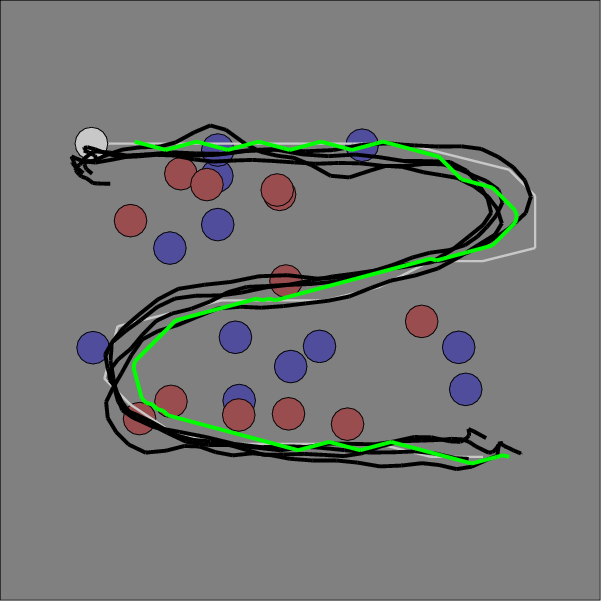
\includegraphics[width=\textwidth]{task_1.png}
\caption{Path module only,\\$w = (0.039, 0.0, 0.960)$. }
\end{subfigure}
\begin{subfigure}[b]{0.24\textwidth}
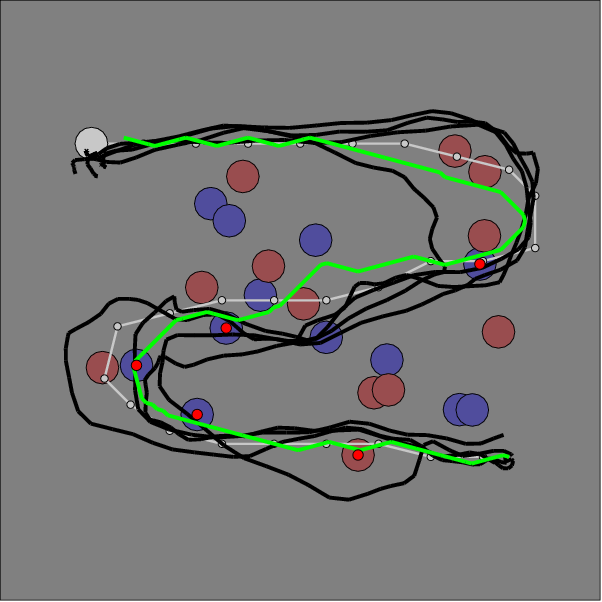
\includegraphics[width=\textwidth]{task_2.png}
\caption{Obstacle + Path,\\$w = (0.081, 0.264, 0.654)$. }
\end{subfigure}
\begin{subfigure}[b]{0.24\textwidth}
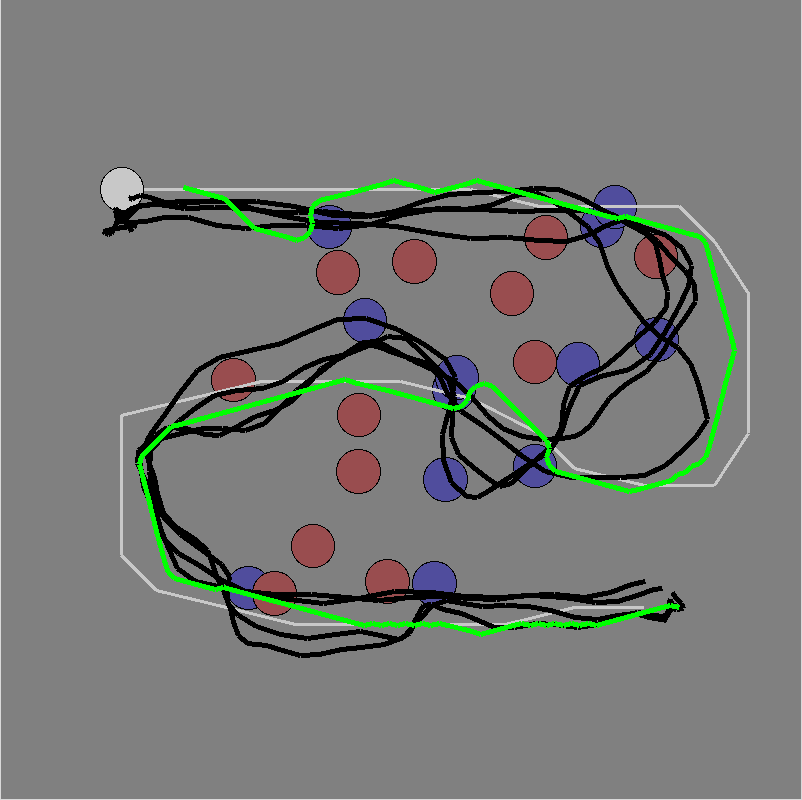
\includegraphics[width=\textwidth]{task_3.png}
\caption{Target + Path, \\$w = (0.254, 0.089, 0.655)$. }
\end{subfigure}
\begin{subfigure}[b]{0.24\textwidth}
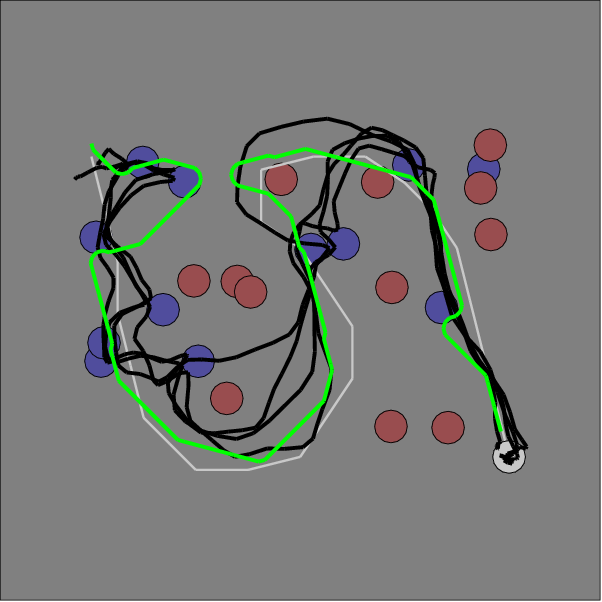
\includegraphics[width=\textwidth]{task_4.png}
\caption{Target + Obstacle + Path, \\$w = (0.215, 0.414, 0.369)$. }
\end{subfigure}
\caption{The trajectories of humans and the agent in the four tasks. Targets are blue and obstacles are red. The
black lines are trajectories of human subjects, and the green lines are
trajectories of the learning agent by using the optimum weights, $w$, derived
from modular inverse reinforcement learning. Weights for each task are given as (target,
obstacle, path).}

\label{fig:exp}
\end{figure}

\begin{figure}[h]
\centering
\begin{subfigure}[b]{0.24\textwidth}
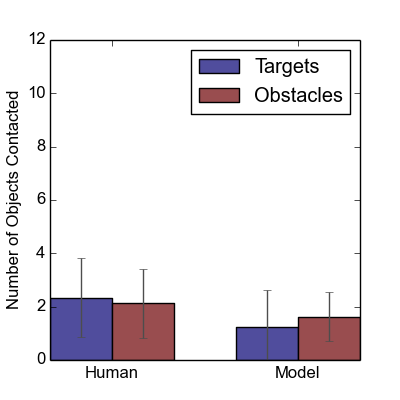
\includegraphics[width=\textwidth]{contact1.png}
\caption{Path module only. }
\end{subfigure}
\begin{subfigure}[b]{0.24\textwidth}
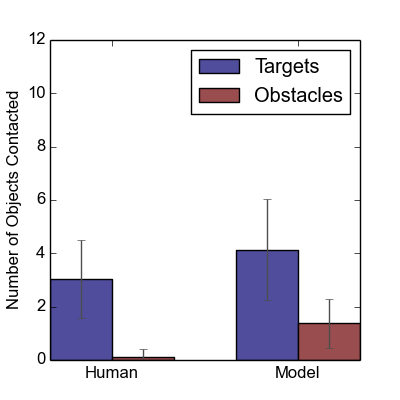
\includegraphics[width=\textwidth]{contact2.png}
\caption{Obstacle + Path. }
\end{subfigure}
\begin{subfigure}[b]{0.24\textwidth}
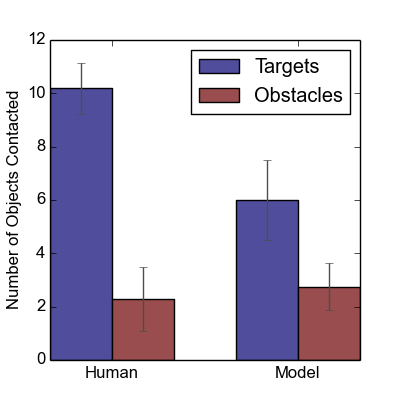
\includegraphics[width=\textwidth]{contact3.png}
\caption{Target + Path. }
\end{subfigure}
\begin{subfigure}[b]{0.24\textwidth}
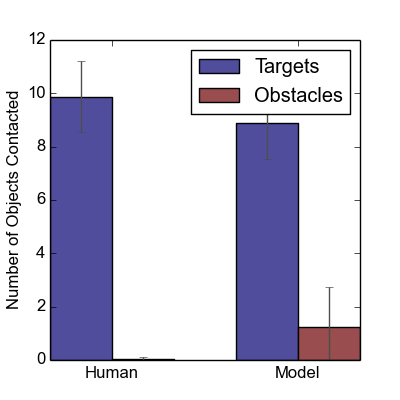
\includegraphics[width=\textwidth]{contact4.png}
\caption{Target + Obstacle + Path. }
\end{subfigure}
\caption{Number of targets hit and number of obstacles hit of the human subjects 
and the agent.}
%COMMENT Shun it would be much better if you used black and green in this figure instead of blue and red since it agree 
%with your previous figure. Also as a side comment its rather obvious that you could do better by using a path constraint that was not so severe
\label{fig:stats}
\end{figure}


The results are shown in Figure~\ref{fig:exp}. As in Figure~\ref{fig:avatar},
the red circles are obstacles and the blue circles are targets. The gray lines
are the path. The black lines are trajectories of individual human subjects,
with each line representing one human trajectory.  Using the weights recovered
by IRL, the trajectories of the agents are drawn in green. Although individual
subjects varied in how they avoided obstacles or collected targets, the agent
can figure out what the humans are doing on aggregate, and perform similarly.
Figure~\ref{fig:stats} evaluates the performance by showing the number of
targets hit and number of obstacles hit.  The number of targets hit should be
large, and the number of obstacles hit should be small, when the corresponding
module is active.  We can observe that humans still do better than the agent in
these tasks.  Nevertheless, the agent performance is quite similar to that of
the human subjects.

\begin{figure}[h]
\centering
\begin{subfigure}[b]{0.4\textwidth}
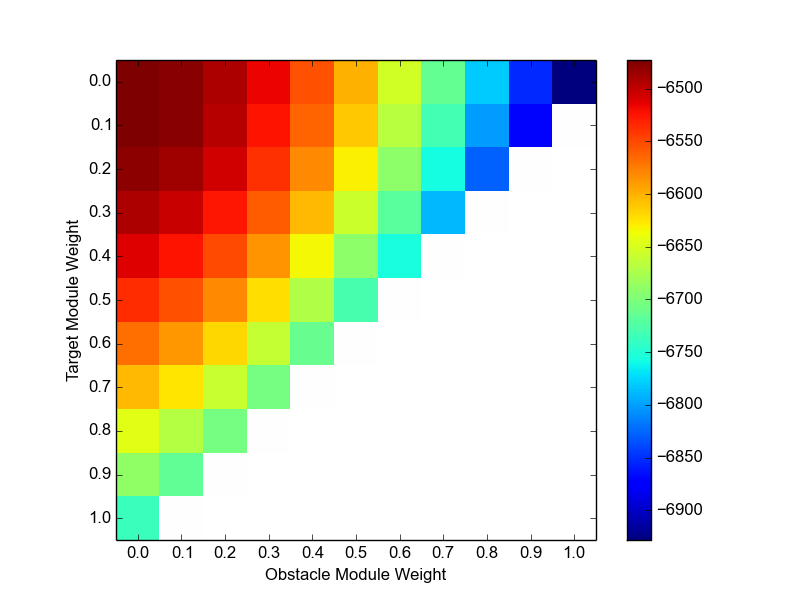
\includegraphics[width=\textwidth]{objValuesTask1.png}
\caption{Path following only.}
\end{subfigure}
\begin{subfigure}[b]{0.4\textwidth}
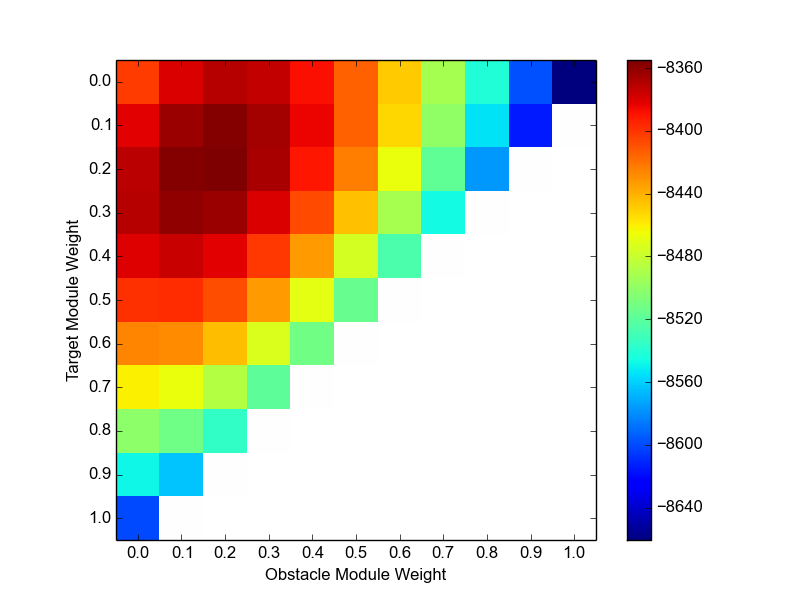
\includegraphics[width=\textwidth]{objValuesTask2.png}
\caption{Obstacle + Path. }
\end{subfigure}
\begin{subfigure}[b]{0.4\textwidth}
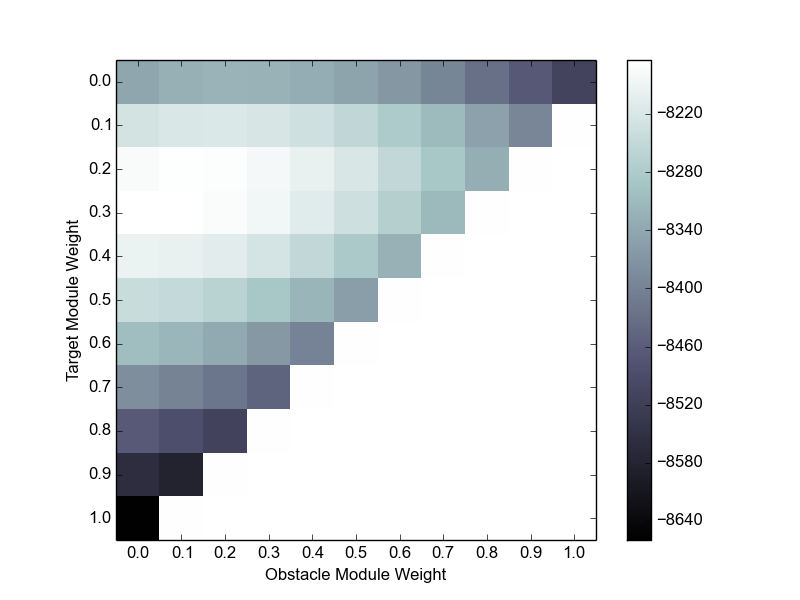
\includegraphics[width=\textwidth]{objValuesTask3.png}
\caption{Target + Path. }
\end{subfigure}
\begin{subfigure}[b]{0.4\textwidth}
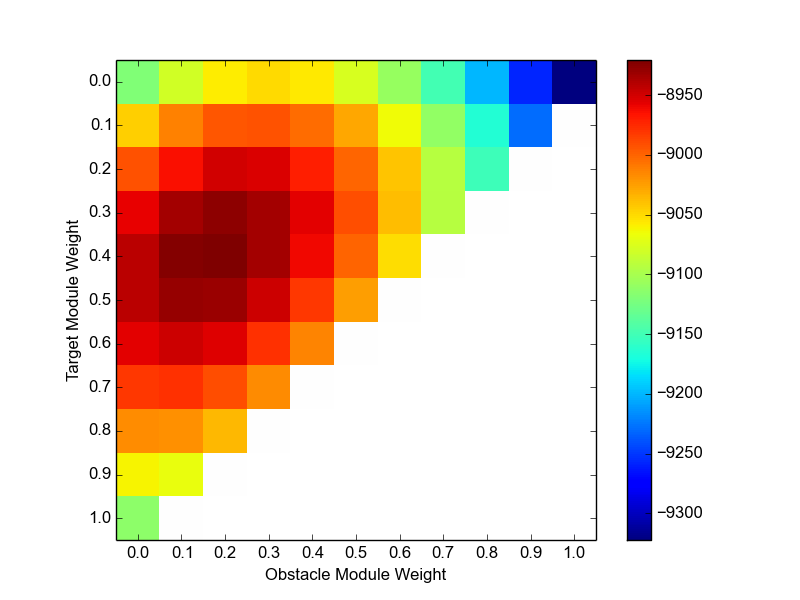
\includegraphics[width=\textwidth]{objValuesTask4.png}
\caption{Target + Obstacle + Path. }
\end{subfigure}
\caption{Heatmaps of the $\log$ of the values of Equation~\ref{eq:irl} for
different weights for the four tasks, respectively. The white zones indicate
higher probabilities. The weights of all three modules sum to 1, so we only show
the weights on the target and the obstacle modules.
}
\label{fig:heatmap}
\end{figure}

In Figure~\ref{fig:heatmap}, we show the $\log$ of values of
Equation~\ref{eq:irl} for different weights. The white color represents higher
probability. We can observe the centroids of white zones move for different
tasks. It stays at the origin in Task 1, so neither the target module nor the
obstacle module is active. It moves away from the origin when a module is
active.  From the heatmaps, we find that fairly well-defined optima exist for
these tasks. The optimal weights are also consistent with the experiment
context.


